\chapter{Computazione quantistica}
\fancyhead[RO, LE]{\bfseries Computazione quantistica}
In questo capitolo si andranno ad approfondire i concetti su cui si basa un computer quantistico, a partire dalla più piccola unità d'informazione, in contrapposizione al bit classico. Si analizzeranno alcune delle sue proprietà fino ad avere una visione d'insieme sia algebrica che geometrica, facendo particolare attenzione alle componenti necessarie per effettuare operazioni con una macchina di questo tipo.

\section{Bit e qubit}
L'unità più piccola d'informazione per i computer classici è il bit: dal punto di vista fisico è un sistema a due stati che può assumere soltanto valore 0 o 1.

Il computer quantistico invece utilizza i qubit \cite{dipierro2013articolo, cambridge2010book} (quantum bit), una particella che si sottomette alle regole della fisica quantistica esistendo in due stati nello stesso istante: potrà assumere sia 1 che 0 contemporaneamente, come mostrato in Figura \ref{fig:bit_qubit}.
\begin{figure}[htp]
    \centering
    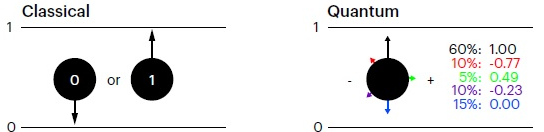
\includegraphics[width=10cm]{Images/Capitolo2/bit_qubit.png}
    \caption{Bit e qubit a confronto.}
    \label{fig:bit_qubit}
\end{figure}

Fu Benjamin Schumacher, presso il Kenyon College (Ohio), che descrisse questo sistema fisico quantistico: più semplice, versatile e potente rispetto a quello digitale.
Per capire la natura di questa entità e la differenza con la sua istanza classica, il bit, dobbiamo fare riferimento alle leggi che regolano il comportamento e l'evoluzione di un sistema fisico reale e di conseguenza l'elaborazione dell'informazione in esso contenuta.

Grazie ad alcuni postulati della meccanica quantistica è stato possibile allargare il campo d'azione di un calcolatore, osservandolo da un'altra prospettiva.
Per questo motivo lo spazio occupato dalle classiche sequenze binarie (registri di bit) includerà tutte le infinite combinazioni (principio di sovrapposizione degli stati) con le loro interazioni non classiche (fenomeno dell'interferenza), che porteranno un effetto sui risultati finali (principio di misurazione) \cite{dipierro2013articolo}.

% Entanglement = Correlazione quantistica
\subsection{Sovrapposizione e entanglement}
Facendo sempre riferimento alla fisica quantistica possiamo identificare il qubit come un vettore $\psi$ nello spazio complesso bidimensionale $\mathbb{C}^2$ (Spazio di Hilbert) definito nella forma
\begin{equation}
    |\psi\rangle = \alpha|0\rangle + \beta|1\rangle =
    \alpha
    \begin{bmatrix}
        0\\
        1
    \end{bmatrix} +
    \beta
    \begin{bmatrix}
        1\\
        0
    \end{bmatrix},
\end{equation}
dove gli scalari $\alpha$ e $\beta$ sono numeri complessi che esprimono l'ampiezza di probabilità dello stato $|0\rangle$ e $|1\rangle$, rispettivamente.
Questi stati intermedi del qubit vengono chiamati sovrapposizioni degli stati e possono essere interpretati come una coesistenza degli stessi in determinate proporzioni: la probabilità che un qubit possa essere 0 oppure 1 è del tutto priva di garanzie e si basa soltanto su situazioni di incertezza.

Esiste inoltre uno stato di correlazione tra due o più sistemi quantistici, che prende il nome di entanglement: in esso due sistemi risultano connessi in un rapporto di causa-effetto, pur non essendo a contatto diretto o indiretto.
A seguito di questo, possiamo introdurre il \say{teletrasporto quantistico} ossia la trasmissione di uno stato quantistico da un punto ad un altro con velocità istantanea \cite{cambridge2010book}.

Entrambi questi fenomeni non sono però sufficienti a fornire una lettura corretta su di un qubit dato che l'informazione trasmessa non si può ritenere certa.
La non-località è un altro principio quantistico dove si afferma che l'entanglement non dipende dalla distanza tra le particelle, le quali possono trovarsi molto lontane tra di loro.

\subsection{Rappresentazione di un qubit nella sfera di Bloch}
All'interpretazione algebrica di un qubit, precedentemente illustrata, possiamo associare anche quella geometrica che ci aiuta ad avere un'intuizione visiva di questa entità, rappresentandola sulla superficie di una sfera unitaria nello spazio reale a tre dimensioni: questa sfera prende il nome dal fisico svizzero Felix Bloch \cite{dipierro2013articolo}.
\begin{figure}[htp]
    \centering
    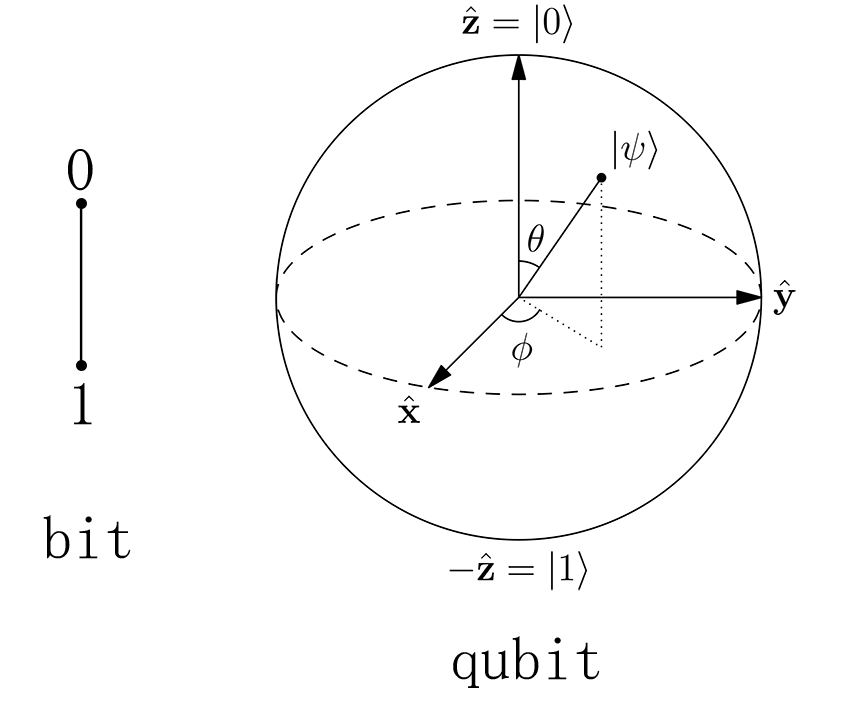
\includegraphics[width=8cm]{Images/Capitolo2/sfera_bloch.png}
    \caption{Interpretazione geometrica bit e qubit.}
    \label{fig:sfera_bloch}
\end{figure}
\newline

Nella Figura \ref{fig:sfera_bloch} possiamo notare come polo nord e polo sud siano associati rispettivamente allo stato quantistico $|0\rangle$ e $|1\rangle$.
Ogni operazione svolta su di un qubit all'interno della sfera, verrà visualizzata come una rotazione all'interno di essa.
Volendo effettuare una rotazione inversa per riportare il punto nella sua posizione originale, anche il qubit può essere invertito e riportato dallo stato finale nello stato iniziale, annullando il suo effetto.

Questa caratteristica prende il nome di reversibilità computazionale e caratterizza fortemente la computazione quantistica.

\subsection{Problema della misurazione quantistica}
Prima di addentrarci nella misurazione di uno stato quantistico introduciamo il concetto di sistema coerente:
\begin{center}
\textit{Un sistema viene definito coerente se determina una fuoriuscita parziale dell'informazione contenuta al suo interno durante l'interazione con un elemento esterno, come ad esempio un misuratore.} \cite{dipierro2013articolo}
\end{center}
Prendendo in considerazione un sistema di piccole dimensioni, come ad esempio un atomo, vogliamo misurare la posizione in cui si trova un elettrone all'interno di esso.

Questo elettrone inizialmente si troverà in una posizione che chiameremo $x$, una volta inserito nel sistema il nostro misuratore possiamo sparare un fotone, così da far muovere l'elettrone che risulterà essere in una nuova posizione che chiameremo $y$.

Possiamo ricondurre questo esempio alla misurazione di un qubit all'interno della sfera di Bloch, ipotizzando di effettuare un qualche tipo di operazione su di esso non avremo modo di misurare coerentemente la sua posizione in quanto si tratta di una misurazione quantistica.
Quest'ultima per essere svolta richiederà la perturbazione del sistema il quale collasserà introducendo determinazione: se ci si trova in uno stato di sovrapposizione la misurazione che andrò a fare ricadrà su uno stato ben preciso e non sulla sovrapposizione stessa.

\section{Porte quantistiche}
I cambiamenti che si verificano in uno stato quantistico possono essere descritti usando il linguaggio del calcolo quantistico.
Come per i computer classici, costituiti da un circuito elettrico contenente fili e porte logiche, così i computer quantistici avranno un circuito quantistico contenente fili e porte quantistiche elementari, in modo da manipolare e trasportare l'informazione quantistica.

L'utilizzo di matrici per rappresentare operazioni lineari \cite{algebra2015book} su di un qubit risulta essere il modo più conveniente.

\subsection{Porte a qubit singolo}
Nei computer classici si può individuare un'unica porta logica (non banale) a un bit, la porta NOT; il cui comportamento può essere completamente descritto dalla sua tabella di verità, dalla quale si evince che l'operazione logica effettuata è quella di una negazione, dove $0\rightarrow1$ e $1\rightarrow0$.

Per definire un'operazione analoga su un qubit, non possiamo limitarci a stabilire la sua azione sugli stati di base $|0\rangle$ e $|1\rangle$, ma dobbiamo specificare anche come deve essere trasformato un qubit che si trova in una sovrapposizione degli stati $|0\rangle$ e $|1\rangle$.
Intuitivamente, il NOT dovrebbe scambiare i ruoli dei due stati fondamentali e trasformare $\alpha|0\rangle + \beta|1\rangle$ in $\alpha|1\rangle + \beta|0\rangle$.
Chiaramente $|0\rangle$ si trasformerebbe in $|1\rangle$ e $|1\rangle$ in $|0\rangle$.

La matrice corrispondente al NOT quantistico, denominata $X$, viene definita come segue:
\begin{equation}
    X=
    \begin{bmatrix}
        0 & 1\\
        1 & 0
    \end{bmatrix}
\end{equation}

L'applicazione di $X$ a un qubit $\alpha|0\rangle + \beta|1\rangle$ risulterà essere:
\begin{equation}
    X
    \begin{bmatrix}
        \alpha \\
        \beta
    \end{bmatrix} =
    \begin{bmatrix}
        \beta \\
        \alpha
    \end{bmatrix}
\end{equation}

Generalmente un'operazione su un singolo qubit può essere rappresentata da una matrice $2\times2$; bisogna però specificare che non tutte le matrici di questo tipo definiscono operazioni \say{lecite} su un qubit; per questo motivo deve essere sempre vera la seguente condizione di normalizzazione \cite{zhao2020articolo}, in qualsiasi stato quantistico esso si trovi:
\begin{equation}
    |\alpha|^2 + |\beta|^2 = 1
\end{equation}

Come abbiamo già detto precedentemente, possiamo definire una sola operazione non banale su un singolo bit, invece per quanto riguarda la computazione quantistica, esistono molte operazioni non banali che agiscono su di un qubit.

Altre due porte di notevole importanza sono la $Z$
\begin{equation}
    Z=
    \begin{bmatrix}
        1 & 0\\
        0 & -1
    \end{bmatrix}
\end{equation}
e la porta Hadamard
\begin{equation}
    H=
    \dfrac{1}{\sqrt{2}}
    \begin{bmatrix}
        1 & 1\\
        1 & -1
    \end{bmatrix}
\end{equation}

La porta $Z$ ha il compito di lasciare invariato lo stato $|0\rangle$ ed invertire il segno dello stato $|1\rangle$ mentre la porta $H$, utilizzata maggiormente, ha il compito di trasformare uno stato base in una sovrapposizione.
L'azione sullo stato $\psi$ sarà quindi definita come segue:
\small
\begin{equation}
    |\psi'\rangle = H
    \begin{bmatrix}
        \alpha\\
        \beta
    \end{bmatrix} =
    \dfrac{1}{\sqrt{2}}
    \begin{bmatrix}
        \alpha + \beta\\
        \alpha - \beta
    \end{bmatrix} =
    \dfrac{1}{\sqrt{2}}
    (\alpha + \beta)|0\rangle +
    \dfrac{1}{\sqrt{2}}
    (\alpha - \beta)|1\rangle
\end{equation}
\normalsize

Per visualizzare l'azione della porta $H$ conviene utilizzare la sfera di Bloch, come mostrato in Figura \ref{fig:hadamard_sfera_bloch}.
Questa porta è rappresentata da una rotazione attorno all'asse $y$ di \ang{90}, seguita da una rotazione attorno all'asse $x$ di \ang{180}.
La sovrapposizione che si genera, dopo una misurazione nella base computazionale, risulta essere $|0\rangle$ oppure $|1\rangle$ con uguale probabilità.
Applicando per esempio $H$ a $|0\rangle$ si ottiene:
\begin{equation}
    H|0\rangle = H
    \begin{bmatrix}
        1\\
        0
    \end{bmatrix} =
    \dfrac{1}{\sqrt{2}}
    \begin{bmatrix}
        1\\
        1
    \end{bmatrix} =
    \dfrac{1}{\sqrt{2}}
    (|0\rangle + |1\rangle)
\end{equation}

L'effetto di $H$ si può quindi vedere come un NOT eseguito a metà, in modo che lo stato risultante non è né 0 né 1, bensì una sovrapposizione dei due stati di base.
Considerando il significato puramente fisico di questa porta si può verificare che $H^2$ è l'identità e quindi applicando due volte $H$ ad uno stato quest'ultimo risulterà inalterato.
Si può provare a visualizzare l'effetto di $H$ sul qubit $\dfrac{1}{\sqrt{2}}(|0\rangle + |1\rangle)$: per effetto della rotazione e della successiva riflessione attraverso il piano $xy$ si otterrà nuovamente $|0\rangle$.

Le matrici $X$, $Z$ e la matrice unitaria
\begin{equation}
    Y=
    \begin{bmatrix}
        0 & -i\\
        i & 0
    \end{bmatrix}
\end{equation}
sono chiamate matrici di Pauli e rappresentano rispettivamente le componenti x, z, y dello spin di un elettrone.
\begin{figure}[htp]
    \centering
    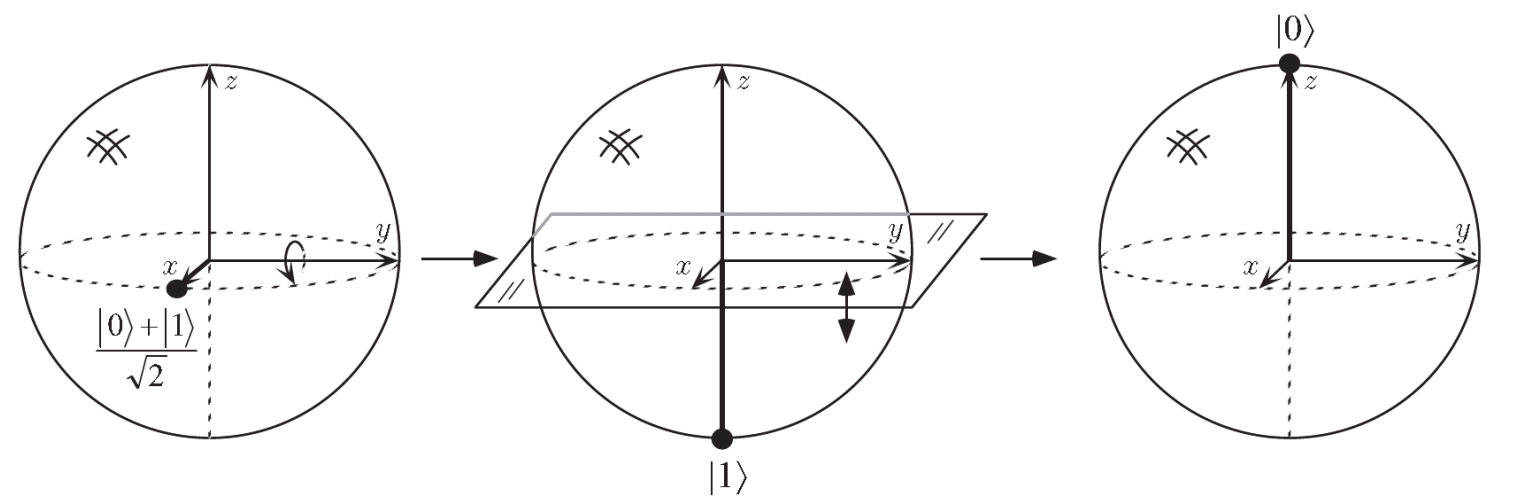
\includegraphics[width=12cm]{Images/Capitolo2/hadamard_sfera_bloch.png}
    \caption{Azione della porta Hadamard sullo stato $(|0\rangle + |1\rangle)/\sqrt{2}$.}
    \label{fig:hadamard_sfera_bloch}
\end{figure}

Prima di introdurre le porte rotazionali è necessario definire la matrice unitaria $u3$, la quale dipende da tre parametri: $\theta, \phi$ e $\lambda$.
\begin{equation}
    \label{eq:u3}
    u3(\theta,\phi,\lambda) =
    \begin{bmatrix}
       \cos{(\theta/2)} & e^{i\lambda}\sin{(\theta/2)}\\
        e^{i\phi}\sin{(\theta/2)} & e^{i\lambda+i\phi}\cos{(\theta/2)}
    \end{bmatrix}.
\end{equation}

Quest'ultima rappresenta una rotazione generica su di un qubit singolo e ci permette inoltre di riportare un qubit nel suo stato precedente.
Come vedremo, valorizzando correttamente questi tre parametri possiamo ottenere le porte rotazionali su tutti e tre gli assi.

Sapendo che qualsiasi matrice unitaria $2\times2$ si può decomporre come
\begin{equation}
    U=e^{i\alpha}
    \begin{bmatrix}
        e^{-i\beta/2} & 0\\
        0 & e^{i\beta/2}
    \end{bmatrix}
    \begin{bmatrix}
        \cos{\frac{\gamma}{2}} & -\sin{\frac{\gamma}{2}}\\
        \sin{\frac{\gamma}{2}} & \cos{\frac{\gamma}{2}}
    \end{bmatrix}
\end{equation}
è possibile costruire una qualsiasi porta a qubit singolo con un numero finito di porte quantistiche in quanto:
\begin{itemize}
    \renewcommand\labelitemi{--}
    \item il primo termine è un fattore di fase globale;
    \item la prima matrice rappresenta una rotazione attorno all'asse $\hat{z}$;
    \item la seconda matrice rappresenta una rotazione attorno all'asse $\hat{y}$.
\end{itemize}

Riuscendo quindi ad implementare le rotazioni attorno a questi assi, sarà possibile realizzare qualsiasi porta a qubit singolo, quindi ogni operazione di rotazione su ogni specifico asse può essere rappresentata con una matrice come raffigurato nelle Equazioni \ref{eq:rx}, \ref{eq:ry}, \ref{eq:rz}.
\begin{equation}
    \label{eq:rx}
    R_x(\theta) =
    \begin{bmatrix}
       \cos{(\theta/2)} & -i\sin{(\theta/2)}\\
        -i\sin{(\theta/2)} & \cos{(\theta/2)}
    \end{bmatrix} =
    u3(\theta,-\pi/2,\pi/2)
\end{equation}
\begin{equation}
    \label{eq:ry}
    R_y(\theta) =
    \begin{bmatrix}
       \cos{(\theta/2)} & -\sin{(\theta/2)}\\
        \sin{(\theta/2)} & \cos{(\theta/2)}
    \end{bmatrix} =
    u3(\theta,0,0)
\end{equation}
\begin{equation}
    \label{eq:rz}
    R_z(\phi) =
    \begin{bmatrix}
       e^{-i\phi/2} & 0\\
        0 & e^{i\phi/2}
    \end{bmatrix} =
    u1(\phi)
\end{equation}
Nella Figura \ref{fig:porte_logice_singolo_qubit} vengono inoltre riassunte e rappresentate graficamente le porte logiche $X$, $Z$ e $H$.
\begin{figure}[htp]
    \centering
    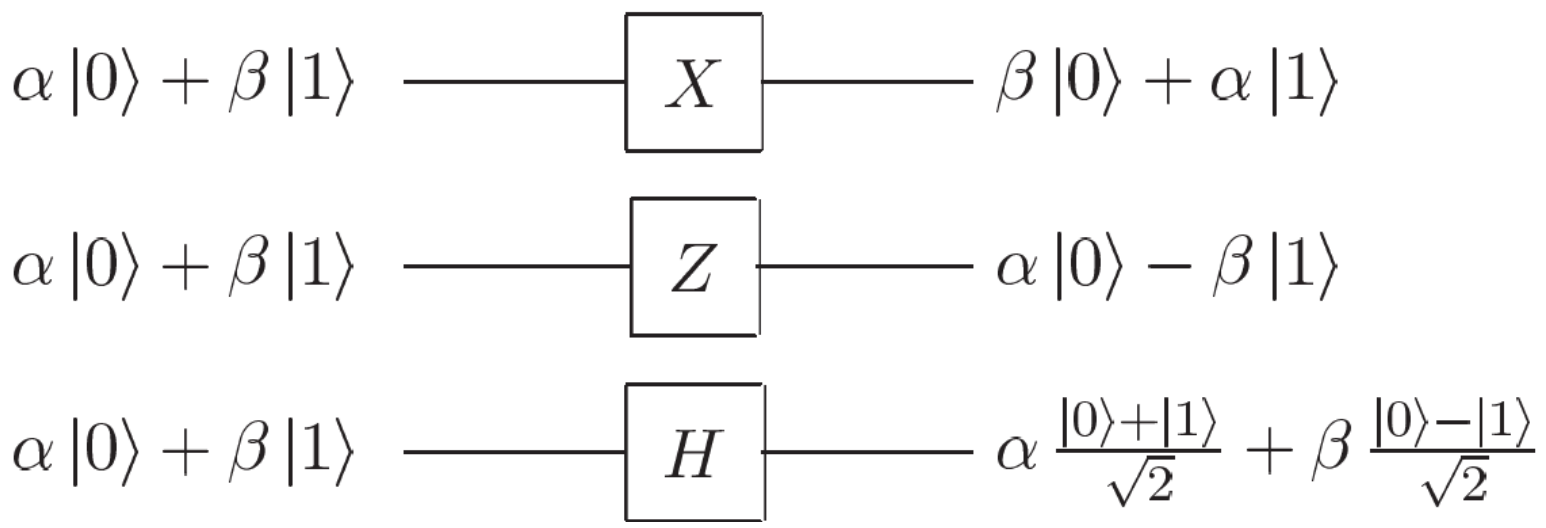
\includegraphics[width=8cm]{Images/Capitolo2/porte_logice_singolo_qubit.png}
    \caption{Esempio di porte a qubit singolo.}
    \label{fig:porte_logice_singolo_qubit}
\end{figure}
\newline
\subsection{Registri quantistici}
Con due bit classici possiamo formare quattro possibili stati: 00, 01, 10, 11.
In generale, con n bit è possibile costruire $2^n$ stati distinti.
Lo spazio degli stati generato da un sistema di n qubit ha dimensione $2^n$: ogni vettore normalizzato in questo spazio rappresenta un possibile stato computazionale, che chiameremo registro quantistico a n qubit.

Questa crescita esponenziale delle dimensioni dello spazio degli stati suggerisce la potenziale capacità di un computer quantistico di elaborare informazioni ad una velocità esponenzialmente superiore rispetto a quella di un computer classico.

Volendo definire formalmente un registro quantistico di n qubit possiamo considerarlo come un elemento dello spazio di Hilbert $2^n$-dimensionale, $\mathbb{C}^{{2}^n}$ con base computazionale formata da $2^n$ registri a n qubit
\begin{equation}
    |i\textsubscript{1}\rangle\otimes|i\textsubscript{2}\rangle\otimes \dotsm \otimes|i\textsubscript{n}\rangle
\end{equation}
con $i\textsubscript{j}\in\{0,1\}, 1 \leq j \leq n$.
Per convenienza il vettore sopra citato verrà scritto come $|i\textsubscript{1}\rangle|i\textsubscript{2}\rangle \dotsm |i\textsubscript{n}\rangle$ oppure $|i\textsubscript{1}i\textsubscript{2} \dotsm i\textsubscript{n}\rangle$.

\subsection{Porte a qubit multipli}
Al fine di implementare operazioni su due bit classici le porte logiche più importanti ed utilizzate sono AND, OR, XOR, NAND, NOR e NOT.

Le porte NOT e AND formano un insieme universale e quindi possono realizzare una qualsiasi funzione booleana, di conseguenza definiremo insieme universale anche la porta NAND.
Non essendo possibile risalire agli input a partire dai risultati, le porte classiche XOR e NAND non sono invertibili, pertanto non è possibile generalizzare le porte classiche a bit multipli con porte quantistiche a qubit multipli.

L'analogo quantistico di una porta universale è il NOT controllato o CNOT (controlled-NOT) che opera su due qubit: il primo è chiamato qubit di controllo mentre il secondo rappresenta il qubit target.
Se il controllo è zero allora il target non viene modificato, altrimenti se il controllo è 1 allora il target viene negato, cioè:
\begin{equation}
    |00\rangle\mapsto|00\rangle, |01\rangle\mapsto|01\rangle, |10\rangle\mapsto|11\rangle, |11\rangle\mapsto|10\rangle.
\end{equation}

Generalizzando una classica porta XOR possiamo vedere la CNOT con la seguente trasformazione:
\begin{equation}
    |A,B\rangle\mapsto|A, B\oplus A\rangle,
\end{equation}
dove $A$ è il qubit di controllo, $B$ è il target e $\oplus$ è la classica operazione XOR.
\begin{figure}[htp]
    \centering
    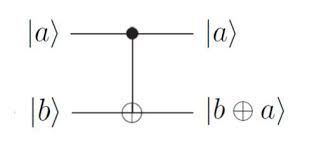
\includegraphics[width=6cm]{Images/Capitolo2/porta_cnot.png}
    \caption{Porta CNOT.}
    \label{fig:porta_cnot}
\end{figure}

Dopo aver visto la rappresentazione grafica del circuito in Figura \ref{fig:porta_cnot} andiamo a descrivere questa porta come matrice unitaria:
\begin{equation}
    CNOT= 
    \begin{bmatrix}
        1 & 0 & 0 & 0\\
        0 & 1 & 0 & 0\\
        0 & 0 & 0 & 1\\
        0 & 0 & 1 & 0
    \end{bmatrix}.
\end{equation}

A differenza delle porte classiche XOR e NAND, la CNOT è invertibile.
Quest'ultima, insieme a quelle a un qubit, rappresenta i prototipi di tutte le porte logiche quantistiche.

\section{Un esempio di circuito}
Ora che abbiamo introdotto tutte le principali porte logiche quantistiche, andiamo ad analizzare un circuito molto utile formato da una porta Hadamard ed una porta CNOT, come mostrato in Figura \ref{fig:circuito_bell}.
\begin{figure}[htp]
    \centering
    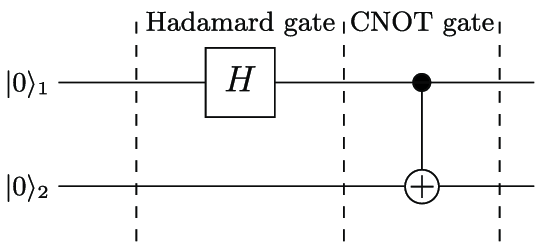
\includegraphics[width=8cm]{Images/Capitolo2/circuito_bell.png}
    \caption{Circuito per creare stati di Bell.}
    \label{fig:circuito_bell}
\end{figure}

Questo circuito trasforma i quattro stati fondamentali del sistema a due qubit in degli stati di Bell \cite{cambridge2010book}, o coppie EPR:
\begin{equation}
    |\beta_{00}\rangle =\dfrac{|00\rangle + |11\rangle}{\sqrt(2)}
\end{equation}
\begin{equation}
    |\beta_{01}\rangle =\dfrac{|01\rangle + |10\rangle}{\sqrt(2)}
\end{equation}
\begin{equation}
    |\beta_{10}\rangle =\dfrac{|00\rangle - |11\rangle}{\sqrt(2)}
\end{equation}\begin{equation}
    |\beta_{1}\rangle =\dfrac{|01\rangle - |10\rangle}{\sqrt(2)}
\end{equation}

La proprietà interessante di questo tipo di stati è che i qubit sono correlati; infatti la misura del secondo qubit restituirà sempre un risultato uguale a quella del primo. Bell dimostrò che questa correlazione viene mantenuta se si effettuano alcune operazioni sulla coppia EPR, prima di svolgere la misurazione dei qubit.

Dato quindi un input specifico, possiamo vedere nella Tabella \ref{table:verita_bell} quale sarà l'output risultante del circuito.
\begin{table}[ht]
\centering
\begin{tabular}{l|c}
    \hline\hline
    \textbf{In} &  \textbf{Out}\\
    \hline
    $|00\rangle$ & {$(|00\rangle + |11\rangle)/\sqrt{2}\equiv |\beta_{00}\rangle$}\\
    $|01\rangle$ & {$(|01\rangle + |10\rangle)/\sqrt{2}\equiv |\beta_{01}\rangle$}\\
    $|10\rangle$ & {$(|00\rangle - |11\rangle)/\sqrt{2}\equiv |\beta_{10}\rangle$}\\
    $|11\rangle$ & {$(|01\rangle - |10\rangle)/\sqrt{2}\equiv |\beta_{11}\rangle$}\\
    \hline\hline
\end{tabular}
\caption{Tabella di verità degli stati di Bell.}
\label{table:verita_bell}
\end{table}

\section{Algoritmi quantistici}
\subsection{Classi di complessità}
Nel mondo della computazione quantistica lo scopo principale è quello di trovare metodi o algoritmi migliori per individuare tutte le possibili soluzioni nella maniera più efficiente.

La teoria che si occupa di stabilire le risorse (tempo o spazio) necessarie per risolvere un determinato problema utilizzando uno specifico algoritmo, prende il nome di complessità computazionale: è quest'ultima a fare la differenza tra computer quantistici e computer classici.

L'obbiettivo è quello di individuare il metodo o l'algoritmo migliore, esplorando così l'intero spazio delle possibili soluzioni nella maniera più efficiente.
Questa problematica risulta essere non banale in quanto, se consideriamo n bit, lo spazio di ricerca contiene un numero di possibili soluzioni nell'ordine di $2^n$.

L'efficienza di un algoritmo è determinata da quanto il problema si presta o meno ad una strutturazione dello spazio delle possibili soluzioni e per misurarla bisogna tenere conto della crescita asintotica del tempo necessario ad ottenere il risultato (es. numero di passi dell'algoritmo) in funzione della dimensione dell'input ed è determinata da molteplici fattori.

Possiamo quindi definire un algoritmo efficiente per la teoria della complessità con uno per cui tale funzione è polinomiale in $n$ e, in corrispondenza, si dirà di ordine $O(n)$, $O(n^2)$, $O(n^3)$ ecc.
\begin{figure}[htp]
    \centering
    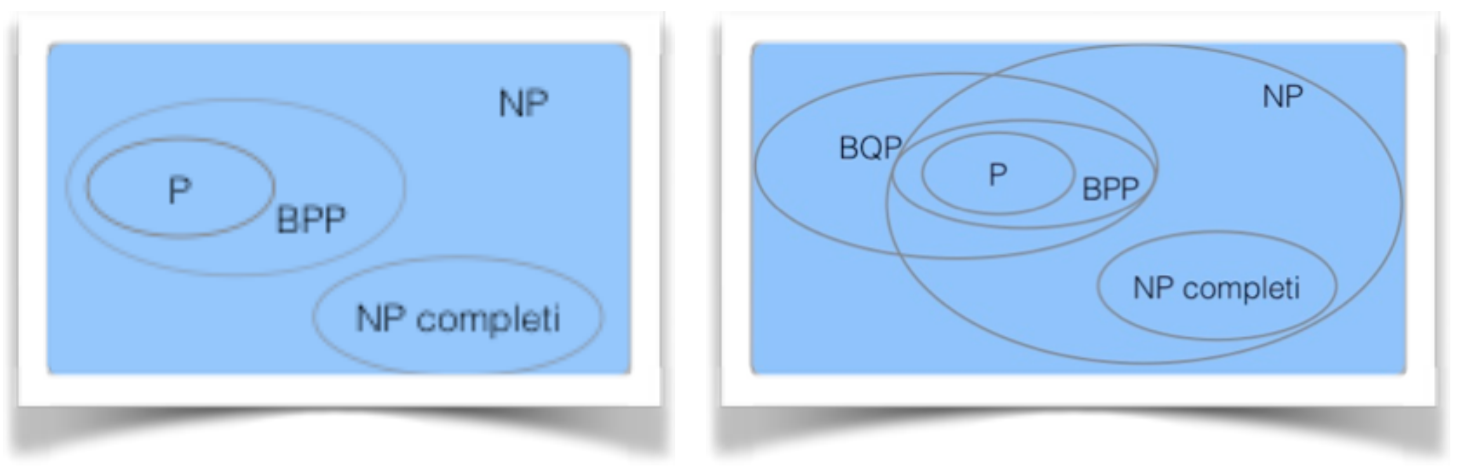
\includegraphics[width=12cm]{Images/Capitolo2/classi_complessita.png}
    \caption{Classi di complessità classiche e con BQP.}
    \label{fig:classi_complessita}
\end{figure}
\newline\newline

Andiamo ora ad approfondire ogni singola classe \cite{dipierro2013articolo}, prendendo come spunto i diagrammi in Figura \ref{fig:classi_complessita}:
\begin{itemize}
    \renewcommand\labelitemi{--}
    \item \textbf{\textit{P (Polynomial-time)}}, classe di tutti i problemi per cui esiste un algoritmo efficiente;
    \item \textbf{\textit{BPP (Bounded-error Probabilistic Polynomial-time)}}, classe dei problemi che possono essere risolti da algoritmi probabilistici in tempo polinomiale, con una probabilità di errore $<\dfrac{1}{3}$;
    \item \textbf{\textit{NP (Nondeterministic Polynomial-time)}}, classe dei problemi che possono essere risolti in tempo polinomiale, purché si utilizzi un algoritmo non deterministico;
    \begin{itemize}
        \item \textbf{\textit{NP completi}}, rappresentano i più difficili problemi non deterministici; un algoritmo in grado di risolvere "velocemente" un qualsiasi problema NP-C può essere utilizzato per risolvere "velocemente" ogni problema in NP;
    \end{itemize}
    \item \textbf{\textit{BQP (Bounded-error Quantum Polynomial-time)}}, classe dei problemi che richiedono da parte di un computer quantistico un tempo polinomiale, con una probabilità di errore $\leq\dfrac{1}{3}$.
\end{itemize}

La relazione presente tra le classi NP e BQP non è attualmente nota, come non è ancora nota l'esistenza di algoritmi efficienti per risolvere problemi NP-C.

\subsection{Teletrasporto quantistico}
Il primo argomento che andremo a trattare non sarà un algoritmo vero e proprio, piuttosto un interessante applicazione dell'elaborazione quantistica dell'informazione ed in particolare dell'entanglement.

Per il teorema di no-cloning quantistico \cite{wootters1982articolo}, copiare lo stato di un qubit è vietato, a meno che esso sia 0 o 1.
Tuttavia, nulla impedisce di teletrasportare \cite{cambridge2010book} il qubit a qualsiasi distanza, anche senza un canale di comunicazione quantistico.

Cerchiamo di fare un esempio considerando due persone fittizie, Alice e Bob.
Insieme, dopo essersi trovati, hanno creato uno stato di Bell.
In seguito si sono separati, prendendo ognuno uno dei due qubit entangled.
Una volta a grande distanza, l'obbiettivo di Alice è trasmettere a Bob, in uno stato sconosciuto, un nuovo qubit $|\psi \rangle=\alpha |0\rangle + \beta |1\rangle$.
Per farlo però, può usare soltanto canali di comunicazione classici (ovvero può spedire solo dei bit).
Grazie ai qubit entangled questo è possibile.

Il circuito è mostrato in Figura \ref{fig:teletrasporto_quantistico}.
Alice crea un sistema con il nuovo qubit e il suo qubit della coppia EPR.
Lo stato iniziale del sistema è
\begin{equation}
    |\psi_0\rangle = |\psi\rangle |\beta_{00}\rangle = \dfrac{1}{\sqrt{2}}[\alpha|0\rangle(|00\rangle + |11\rangle)+\beta|1\rangle(|00\rangle + |11\rangle)],
\end{equation}
dove i primi due qubit (sinistra) sono di Alice ed il terzo è di Bob.
Alice manda i suoi qubit in una porta CNOT, ottenendo
\begin{equation}
    |\psi_1\rangle = \dfrac{1}{\sqrt{2}}[\alpha|0\rangle (|00\rangle + |11\rangle)+\beta|1\rangle (|10\rangle + |01\rangle)].
\end{equation}

Alice manda poi il suo primo qubit in una porta Hadamard, ottenendo
\begin{equation}
    |\psi_2\rangle = \dfrac{1}{\sqrt{2}}[\alpha(|0\rangle + |1\rangle)(|00\rangle + |11\rangle) + \beta(|0\rangle - |1\rangle)(|10\rangle + |01\rangle)].
\end{equation}

Se raccogliamo i qubit di Alice, possiamo riscrivere l'equazione come
\begin{equation}
    \begin{split}
    |\psi_2\rangle =
    &\dfrac{1}{\sqrt{2}}[|00\rangle (\alpha|0\rangle + \beta|1\rangle)+|01\rangle(\alpha|1\rangle+\beta|0\rangle)+\\&+|10\rangle(\alpha|0\rangle-\beta|1\rangle)+|11\rangle(\alpha|1\rangle-\beta|0\rangle)].
    \end{split}
\end{equation}

A questo punto, Alice misura i suoi due qubit e manda il risultato a Bob. A seconda del risultato ottenuto, il sistema si troverà in uno di questi quattro stati:
\begin{gather}
 00 \longmapsto |\psi_3(00)\rangle = [\alpha|0\rangle + \beta|1\rangle]\\
 01 \longmapsto |\psi_3(01)\rangle = [\alpha|1\rangle + \beta|0\rangle]\\
 10 \longmapsto |\psi_3(10)\rangle = [\alpha|0\rangle - \beta|1\rangle]\\
 11 \longmapsto |\psi_3(11)\rangle = [\alpha|1\rangle - \beta|0\rangle]
\end{gather}

Per recuperare lo stato $\psi$ Bob deve applicare una porta quantistica che dipende dal risultato spedito da Alice.
Se il risultato è 00, Bob non deve applicare nulla.
Se il risultato è 01, Bob deve applicare una porta $X$.
Se il risultato è 10, Bob deve applicare una porta $Z$.
Se il risultato è 11, Bob deve applicare una porta $X$ e poi una porta $Z$.

Per riassumere, Bob deve applicare una porta $Z^{M_1}X^{M_2}$ (dove $M_1$ e $M_2$ sono i due bit inviati da Alice, e come nel prodotto matriciale viene applicato prima il termine sulla destra).
\begin{figure}[htp]
    \centering
    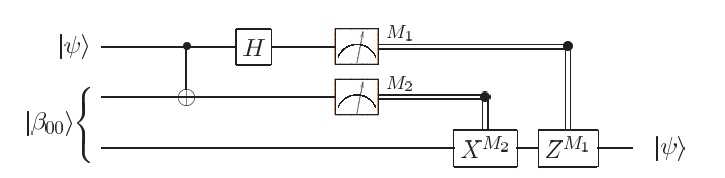
\includegraphics[width=13cm]{Images/Capitolo2/teletrasporto_quantistico.png}
    \caption[Circuito quantistico per il teletrasporto di un qubit.]{Circuito quantistico per il teletrasporto di un qubit. Le prime due linee rappresentano i qubit di Alice, mentre la terza il qubit di Bob.}
    \label{fig:teletrasporto_quantistico}
\end{figure}

Uno degli utilizzi più frequenti del teletrasporto quantistico, in ambito di computazione quantistica, riguarda la creazione di porte quantistiche che resistano al rumore.

\subsection{VQE}
\label{subsec:vqe}
L'algoritmo Variational Quantum Eigensolver (VQE) utilizzato nella fase sperimentale, che andremo ad implementare nell'Appendice \ref{codice:vqe}, ha l'obbiettivo di stimare le proprietà molecolari di un sistema quantistico utilizzando il principio variazionale.

Una proprietà molto spesso analizzata riguarda lo stato fondamentale di un atomo o di una molecola: l'utilizzo frequente di questo algoritmo ibrido trova applicazione nel campo della chimica computazionale quantistica.
Si definisce ibrido in quanto utilizza cicli alternati di calcolo classico e quantistico: nello specifico ci consente di trovare l'autovalore di una matrice H (solitamente di grandi dimensioni) attraverso una tecnica chiamata media Hamiltoniana.

Questa tecnica, in presenza di molti corpi, risulta difficile da studiare nei computer classici a causa della sua complessità e dimensionalità, mentre nei computer quantistici si hanno meno problemi di sovraccarico con conseguente crescita polinomiale.
Possiamo quindi schematizzare l'algoritmo VQE \cite{chimica_quantistica} nei seguenti passaggi:
\begin{enumerate}
    \item \textbf{\textit{Preparazione dello stato}}: uno stato quantistico parametrizzato $|\psi(\Vec{\theta})\rangle$ è preparato sul dispositivo quantistico. Questo grazie all'applicazione di un parametro unitario definito dalla scelta dell'\textit{ansatz}, il quale dovrebbe contenere una famiglia di stati non rappresentabili in maniera efficiente su di un computer classico;
    \item \textbf{\textit{Stima energetica}}: il valore atteso dall'energia $\langle H\rangle(\theta)$ è stimato utilizzando la procedura della media Hamiltoniana, la quale prevede la misurazione di prodotti tensoriali in termini di Pauli, corrispondenti alla rappresentazione del qubit;
    \item \textbf{\textit{Feedback classico}}: i parametri dello stato quantistico $\Vec{\theta}$ vengono aggiornati utilizzando una routine classica non lineare;
    \item I punti 2 e 3 vengono ripetuti finché i criteri di convergenza non sono soddisfatti.
\end{enumerate}

La struttura di base di VQE, rappresentata in Figura \ref{fig:struttura_vqe}, può essere definita modulare, in quanto lascia possibilità di futuri miglioramenti ed estensioni.
\begin{figure}[htp]
    \centering
    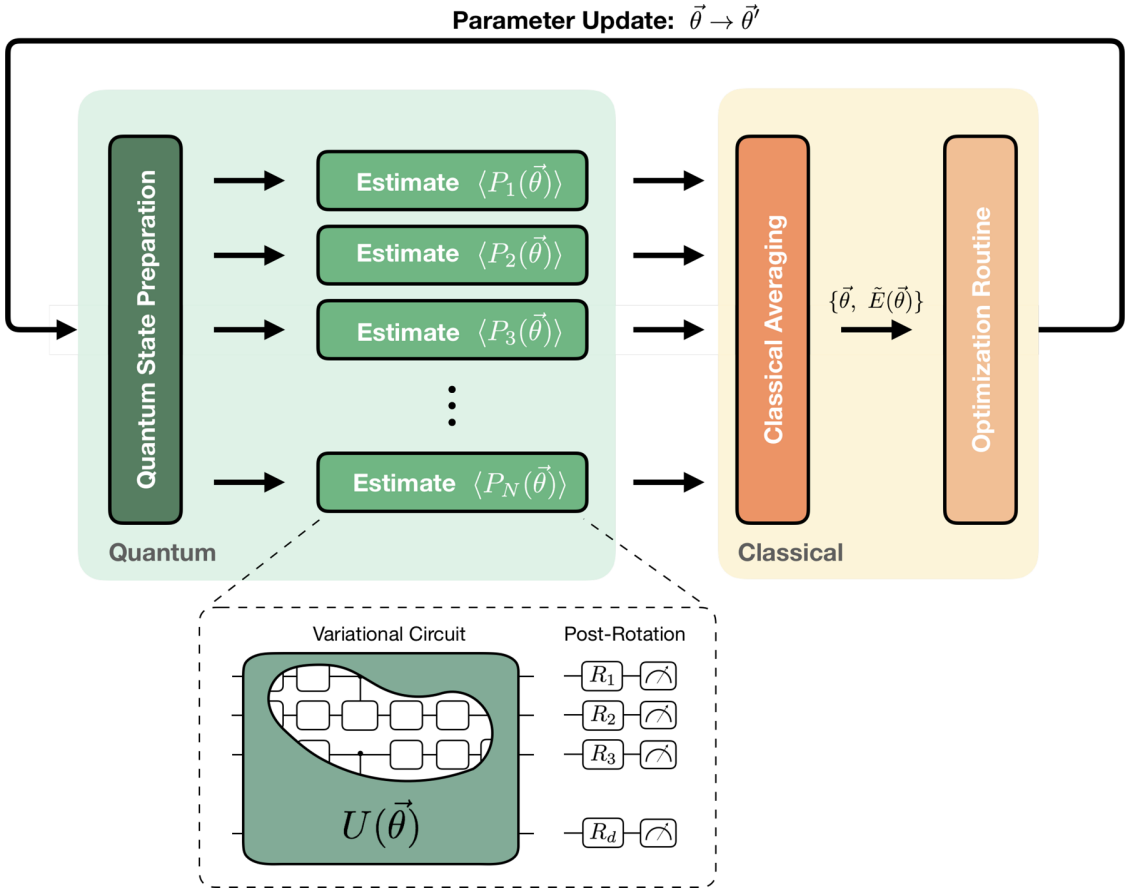
\includegraphics[width=\textwidth]{Images/Capitolo2/struttura_vqe.png}
    \caption{Illustrazione algoritmo VQE.}
    \label{fig:struttura_vqe}
\end{figure}
\newline\newline

\subsubsection{Equazione di Schrödinger}
Per introdurre questo argomento, dobbiamo prima definire il concetto di principio variazionale utilizzato nel paragrafo precedente; in generale questa tecnica ha lo scopo di risolvere un problema scientifico utilizzando il calcolo delle variazioni.

Nel nostro caso, parlando di meccanica quantistica \cite{sakai2018equazione}, quando calcoliamo il valore medio dell'operatore Hamiltoniano su una funzione d'onda arbitraria possiamo affermare che questo valore non sarà mai inferiore all'energia dello stato fondamentale.

Questo metodo risolve dunque l'equazione di Schrödinger (\ref{eq:equazione_schrodinger}), la quale rappresenta una delle più importanti conquiste della fisica ed in particolare della meccanica quantistica, consentendoci di trovare la \textit{funzione d'onda}, seno o coseno, che descrive il comportamento di una particella microscopica.
In termini più semplici, grazie ad essa riusciamo a calcolare le probabilità di trovare un elettrone nello spazio intorno al nucleo.

Definendo quindi l'Equazione \ref{eq:equazione_schrodinger} di Schrödinger e l'energia classica espressa come Hamiltoniana nell'Equazione \ref{eq:energia_hamiltoniana}, possiamo riscrivere la prima in maniera compatta:
\begin{equation}
    \label{eq:equazione_schrodinger}
    H(t)|\psi(t)\rangle=i\hbar\dfrac{\partial}{\partial t}|\psi(t)\rangle,
\end{equation}
\begin{equation}
    \label{eq:energia_hamiltoniana}
    H=\dfrac{p^{2}}{2m}+V(x),
\end{equation}
\begin{equation}
    \label{eq:sistema_qualsiasi_schrodinger}
    -\dfrac{\hbar^{2}}{2m}\dfrac{d^{2}\psi (x)}{dx^{2}}+V\psi (x)=E\psi (x),
\end{equation}
\begin{equation}
    \hat{H}\psi = E\psi,
\end{equation}
dove $\hat{H}$ rappresenta l'operatore Hamiltoniano.